\documentclass[a4paper,10pt]{article}

%{{{ packages
\usepackage{blindtext}
\usepackage{lipsum}
\usepackage[ngerman]{babel}
\usepackage[tiny]{titlesec}
\usepackage{index}
\usepackage[onehalfspacing]{setspace}
\usepackage{fullpage}
\usepackage{pdfpages}
\usepackage{fancyhdr}
\usepackage{authblk}
\usepackage{hyperref}
\hypersetup{colorlinks=true,allcolors=blue}

%\usepackage{tabulary}
%\usepackage{tabularx}
\usepackage{booktabs}%toprule,midrule,bottomrule
\usepackage{multirow}
\usepackage{multicol}
\usepackage{tikz}
\usepackage[european,siunitx]{circuitikz}
\usepackage{graphicx}
\usepackage{svg} %\includesvg{}
\usepackage{import} % can import files from other directories
\usepackage{longtable}
\usepackage{pgfplots}
\usepackage{gnuplottex}
\usepackage{wrapfig}

\usepackage{amsmath,amsfonts,amssymb}
\usepackage{tensor} %for indices
\usepackage{dsfont} % double stroke font
\usepackage{cancel} % cancel in frac
\usepackage{bm} % bold math font (if error is produced use \bm{{}})
\usepackage{mathtools}
\usepackage[ISO]{diffcoeff}
\usepackage[locale=DE]{siunitx}
\usepackage[official]{eurosym}
%\usepackage{mathrsfs} % calligraphy font
\usepackage{physics}
\usepackage[a]{esvect}
\usepackage{bigints}
%\usepackage[frak=esstix]{mathalpha} % disable if LaTeX uses too many alphabets
\usepackage{siunitx}
\usepackage[ruled,vlined,linesnumbered]{algorithm2e}
\usepackage{listings}

\usepackage{babel}
\usepackage{hyphsubst}
\usepackage[figurename=Fig.]{caption}
\usepackage{xr} % crossreferencing between documents \externaldocument{}
\usepackage{enumitem} % for enumerate environment
\usepackage{lineno}
\usepackage{makecell}
\usepackage{xcolor}
\usepackage{color}

\allowdisplaybreaks % allows equations to be broken (e.g. by multicols)

\usetikzlibrary{arrows}
\pgfplotsset{compat=1.15}

\newcommand{\td}{\,\text{d}}
\newcommand{\RN}[1]{\uppercase\expandafter{\romannumeral#1}}
\newcommand{\zz}{\mathrm{Z\kern-.3em\raise-0.5ex\hbox{Z} }}
\newcommand{\id}{\mathds{1}}

\newcommand\inlineeqno{\stepcounter{equation}\ {(\theequation)}}
\newcommand\inlineeqnoa{(\theequation.\text{a})}
\newcommand\inlineeqnob{(\theequation.\text{b})}
\newcommand\inlineeqnoc{(\theequation.\text{c})}

\newcommand\inlineeqnowo{\stepcounter{equation}\ {(\theequation)}}
\newcommand\inlineeqnowoa{\theequation.\text{a}}
\newcommand\inlineeqnowob{\theequation.\text{b}}
\newcommand\inlineeqnowoc{\theequation.\text{c}}

\renewcommand{\refname}{Source}
\renewcommand{\sfdefault}{phv}

\newenvironment{Figure}
  {\par\medskip\noindent\minipage{\linewidth}}
  {\endminipage\par\medskip}% for multicols figures
%\pagestyle{fancy}

\sloppy

\numberwithin{equation}{section}

\titleformat{\subsection}{}{\thesubsection}{1em}{\itshape}
\titleformat{\subsubsection}{}{\thesubsubsection}{1em}{\itshape}

%}}}

\begin{document}

%{{{ Titelseite

\begin{titlepage}
  \title{Statistical Mechanics}
  \author{Jonas Wortmann\thanks{s02jwort@uni-bonn.de}}
  \affil{Rheinische Friedrich--Wilhelms--Universität Bonn}
\end{titlepage}

\maketitle
\pagenumbering{arabic}

\renewcommand\abstractname{Abstract}
\abstract{\noindent This work is a short summary on the derivation of the methods of statistical mechanics as well as its application to various systems whether they be discrete or continuous.
The focus is on ensemble theory.
The derivations and arguments rely heavily on \textsc{Raj Kumar Pathria} \textit{Statistical Mechanics} as well as \textsc{Nicolas Borghini} \textit{Statistische Physik} script (Bielefeld) and \textsc{Johann Kroha}'s lecture (Bonn WS24/25).}

%}}}

%\clearpage

%{{{ Inhaltsverzeichnis

\fancyhead[R]{\leftmark}
%\fancyhead[R]{\leftmark\\\rightmark}
\fancyhead[L]{\thepage}
\fancyfoot[C]{}

\renewcommand\contentsname{Contents}
\tiny
\tableofcontents
\normalsize

%}}}

%\clearpage

\vspace{1em}
\hrule

\begin{multicols}{2}

% {{{ Ensemble Theory
\section{Ensemble Theory}
Imagine one would like to study the microscopic behaviour of a many particle system.
It is impossible to solve the equations of motions for every particle analytically, thus one has to rely on probability theory and statistical mechanics.
For a system one can therefore measure macroscopic quantities e.g.\ pressure, volume or temperature.
A set of these quantities with certain values makes out the macrostate of the system.
On the microscopic scale (i.e.\ positions, momenta) however, it is possible to realize this macrostate in many ways.
A state which realizes a certain macrostate is called a microstate $\left(=:\mathfrak{m}\right)$.
There is often more than one microstate to correspond to / realize a certain macrostate.
For a many particle system made up of $N$ particles, a microstate is a single point in a $6N$ dimensional phase space with $3N$ positions and $3N$ momenta.
The time evolution is a single curve through this phase space, thus a series of different microstates (which each have to realize the same macrostate).
One can imagine a gas inside a box: The positions of all gas particles will change over time however the volume will always stay the same.

To study the macrostate from a microstate one can take a time average of all microstates, which have been on the trajectory.
For example the average value of an observable $f$ is given by
\begin{align} 
  \left\langle f \right\rangle _t=\lim_{t\rightarrow \infty}\dfrac{1}{t}\int_{0}^{t}\td t'\,f(t')
.\end{align} 
To compute this integral one has to know the time dependence of $f$. 
Instead one could also make use of the ergodic theorem and average a multitude of identically prepared system to achieve the same average.
The theorem states that a dynamical system will eventually visit all parts of its phase space
\footnote{A more rigorous explanation is definitely needed, but the general picture is clear.}.
Together with Liouville's theorem, if a system is prepared, such that it uniformly fills its phase space, then the system will always have the same phase space distribution.
Since a single system will visit all parts of its phase space over an arbitrarily long period of time, one can achieve the same goal by preparing infinitely many identical systems, which are all left to themselfes to evolve through time hence will also visit all parts of phase space, and take the average over all these systems at a certain instant in time.
\begin{align} 
  \left\langle f \right\rangle _e=\sum_{\mathfrak{m}}^{}p_\mathfrak{m} f = \left\langle f \right\rangle _t
,\end{align} 
whereby $p_\mathfrak{m}$ is the probability that a certain microstate $\mathfrak{m}$ is realized in any system.
The set of all identically prepared systems are called an ensemble.
These systems are, in general, only imaginary copies of a single system and they are considered in the calculation as possible microstates for that system (i.e.\ they don't have to be considered as a separate system for which there are neccessary calculation to do).
The use of this theory is not apparent when one considers a precisely known macroscopic system i.e.\ all macrostates are fixed.
However, if one only fixes a certain amount of macrostates and leaves e.g.\ the energy to be arbitrary, then the restriction on the phase space trajectory is lifted in that dimension and the microstates allow for an arbitrary range of energies within the hyperplane conformal to its restriction.
Then one can utilise the methods of the theory to calculate the average energy of such a system by summing over all energies (which are realized in a certain microstate) and weighing them with a probability function.
%}}}

%{{{ Probability Distribution and Partition Sum
\section{Probability Distribution and Partition Sum}

%{{{ Derivation
\subsection{Derivation}
Imagine a certain set of available data or information about a probability distribution:
To derive the underlying distribution function, the best model is the one, which only assumes the least amount of knowledge about it.
Thus, to find a suitable probability distribution which models the microstates for a given macrostate one maximizes the entropy (principle of maximal entropy), since the entropy encodes the lack of information on a system (or, in this case, is proportional to the amount of available microstates).

The entropy is given by
\begin{align} 
  \boxed{S = -k_B\sum_{i}^{}p_i \ln p_i\equiv -k_B\text{tr}\left(\rho \ln \rho \right)}
,\end{align} 
with $p_i$ being the probability that the $i^{\text{th}}$ microstate\footnote{The label is equivalent $\mathfrak{m}\equiv i$ but the sum over $i$ is more common.} is realized and $\rho $ being the density matrix.
The only constraints are that the probability distribution may be normalized and that it is used to calculate the average value of any observable $A^l$ 
\begin{align} 
  f_0 &= \sum_{i}^{}p_i-1=0 & f_l &= \sum_{i}^{}p_iA^l-\left\langle A^l\right\rangle =0
,\end{align} 
while the sum of $f_l$ ranges over all $i$ microstates.
The Lagrangian is
\begin{align} 
  \mathcal{L} &= S - k_B\lambda _0f_0 - k_B\sum_{l}^{}\lambda _lf_l\\
              &\begin{multlined}
              = -k_B\sum_{i}^{}p_i\ln p_i - k_B\lambda _0\left(\sum_{i}^{}p_i-1\right) \\- k_B\sum_{l}^{}\lambda _l\left(\sum_{i}^{}p_iA^l-\left\langle A^l\right\rangle \right)
              \end{multlined}
.\end{align} 
Now taking the variation w.r.t.\ to all $p_i$ equal to zero
\begin{multline}
  \delta _{p_i}\mathcal{L} = k_B\left(-\sum_{i}^{}\ln p_i - \sum_{i}^{}1 - \lambda _0\sum_{i}^{}1 \right.\\ -\left.\sum_{l}^{}\lambda _l \sum_{i}^{}A^l\right)\delta p_i=0
.\end{multline}
Exchanging $\sum_{l}^{}$ and $\sum_{i}^{}$ in the last term and taking $\sum_{i}^{}$ out of the parentheses yields
\begin{align} 
  -\ln p_i - 1 - \lambda _0 - \sum_{l}^{}\lambda _lA^l &= 0
,\end{align} 
because $\delta _{p_i}\mathcal{L}=0\,\forall \delta p_i$ independently.
\begin{align} 
  p_i &= \text{e}^{-(1 + \lambda _0) - \sum_{l}^{}\lambda _lA^l} = \text{e}^{-(1+\lambda _0)}\text{e}^{-\sum_{l}^{}\lambda _lA^l}
.\end{align} 
The normalisation multiplier yields
\begin{align} 
  \sum_{i}^{}p_i &= \sum_{i}^{}\text{e}^{-(1+\lambda _0)}\text{e}^{-\sum_{l}^{}\lambda _lA^l}\\
                 &= \text{e}^{-(1+\lambda _0)}\sum_{i}^{}\text{e}^{-\sum_{l}^{}\lambda _lA^l}\\
                 &= 1\\
  \Leftrightarrow \text{e}^{-(1+\lambda _0)} &= \dfrac{1}{\sum_{i}^{}\text{e}^{-\sum_{l}^{}\lambda _lA^l}}=:\dfrac{1}{Z}
.\end{align} 
Thereby
\begin{align} 
  \boxed{p_i=\dfrac{\text{e}^{-\sum_{l}^{}\lambda _lA^l}}{\sum_{i}^{}\text{e}^{-\sum_{l}^{}\lambda _lA^l}}=:\dfrac{\text{e}^{-\sum_{l}^{}\lambda _lA^l}}{Z}}
.\end{align} 
The other Lagrange multiplier yields
\begin{align} 
  \sum_{i}^{}p_iA^l &= \sum_{i}^{}\dfrac{\text{e}^{-\sum_{l}^{}\lambda _lA^l}}{\sum_{i}^{}\text{e}^{-\sum_{l}^{}\lambda _lA^l}}A^l\\
                      &= \dfrac{1}{Z}\sum_{i}^{}\text{e}^{-\sum_{l}^{}\lambda _lA^l}A^l\\
                      &= -\dfrac{1}{Z}\diffp*[]{\sum_{i}^{}\text{e}^{-\sum_{l}^{}\lambda _lA^l}}{\lambda _l}\\
                      &= \boxed{-\diffp[]{\ln Z}{\lambda _l} = \left\langle A^l\right\rangle }
.\end{align} 
The relation $-\diffp[]{\ln Z}{\lambda _l} = \left\langle A^l\right\rangle $ is used to determine the Lagrange multiplier.
It is also useful to know
\begin{align} 
  \left\langle A^2\right\rangle  &= \sum_{i}^{}\dfrac{\text{e}^{-\sum_{l}^{}\lambda _lA^l}}{\sum_{i}^{}\text{e}^{-\sum_{l}^{}\lambda _lA^l}}{A^l}^2\\
                                 &= \dfrac{1}{Z}\diffp[2]{Z}{\lambda _l}\\
                                 &= \diffp*[]{\left(\dfrac{1}{Z}\diffp[]{Z}{\lambda _l}\right)}{\lambda _l}-\diffp*[]{\dfrac{1}{Z}}{\lambda _l}\diffp[]{Z}{\lambda _l}\\
                                 &= \diffp[2]{\ln Z}{\lambda _l}+\dfrac{1}{Z^2}\diffp[]{Z}{\lambda _l}\diffp[]{Z}{\lambda _l}\\
                                 &= \diffp[2]{\ln Z}{\lambda _l}+\left(\diffp[]{\ln Z}{\lambda _l}\right)^2\\
  \Leftrightarrow \diffp[2]{\ln Z}{\lambda _l} &= \left\langle {A^l}^2\right\rangle -\left\langle A^l\right\rangle ^2 = \text{Var}\left(A^l\right)
\end{align}
in general
\begin{align} 
  \diffp[]{\ln Z}{\lambda _k,\lambda _l} &= \left\langle A^lA^k\right\rangle -\left\langle A^l\right\rangle \left\langle A^k\right\rangle 
.\end{align}
Recall the general formula for entropy
\begin{align} 
  S &= -k_B\sum_{i}^{}p_i\ln p_i\\
    &= -k_B\left\langle \ln p_i\right\rangle \\
    &= k_B\left\langle \ln Z\right\rangle -k_B\left\langle \ln \text{e}^{-\sum_{l}^{}\lambda _lA^l}\right\rangle \\
    &= k_B\ln Z + k_B\left\langle \sum_{l}^{}\lambda _lA^l\right\rangle \\
  \Aboxed{S &= k_B\ln Z + k_B\sum_{l}^{}\lambda _l\left\langle A^l\right\rangle }\\
    &= k_B\ln Z - k_B\sum_{l}^{}\lambda _l\diffp[]{\ln Z}{\lambda _l}
,\end{align} 
Consider the derivative of $S$ w.r.t.\ $\left\langle A^l\right\rangle $ and choose $A^l=E$ with $\lambda _l=\beta $ as the energy
\begin{align} 
  \diffp[]{S}{\left\langle E\right\rangle } &= k_B\beta =\dfrac{1}{T}\Leftrightarrow \boxed{\beta =\dfrac{1}{k_BT}}
\end{align} 
by comparison with the thermodynamic potential of the entropy and its derivatives
\footnote{The assumption $U=\left\langle E\right\rangle $ is phenomenological.}.
If one were to set $A^l=N$ and $\lambda _l=-\alpha $ as the particle number
\begin{align} 
  \diffp[]{S}{\left\langle N\right\rangle }=-k_B\alpha =-\dfrac{\mu }{T}\Leftrightarrow \boxed{\alpha =\dfrac{\mu }{k_BT}}
.\end{align} 
This can also be derived from the total differential of $S$.
\begin{align} 
  \td S &= -\td \left(k_B\sum_{i}^{}p_i\ln p_i\right)\\
        &= -k_B\sum_{i}^{}\left(\ln p_i + 1\right)\td p_i
.\end{align} 
$\sum_{i}^{}\td p_i=0$ due to the normalisation constraint.
In the canonical ensemble $p_i = \tfrac{1}{Z}\text{e}^{-\beta E}$
\begin{align} 
  \td S &= k_B\sum_{i}^{}\left(\ln Z + \beta E\right)\td p_i\\
        &= k_B\beta \sum_{i}^{}E\td p_i
,\end{align}
since $Z$ is a number.
Compare the first law of thermodnamics
\begin{align} 
  \td S &= \dfrac{1}{T}\td \left\langle E\right\rangle  + \dfrac{p}{T}\td V\\
        &= \dfrac{1}{T}\td \left(\sum_{i}^{}p_iE\right) + \dfrac{p}{T}\td V\\
        &= \dfrac{1}{T}\left(\sum_{i}^{}E\td p_i + \sum_{i}^{}p_i\td E\right) + \dfrac{p}{T}\td V\\
        &= \dfrac{1}{T}\sum_{i}^{}E\td p_i + \dfrac{1}{T}\left\langle \td E\right\rangle +\dfrac{p}{T}\td V\\
  \td S &= k_B\beta \sum_{i}^{}E\td p_i
,\end{align} 
which yields
\begin{align} 
  \beta  &= \dfrac{1}{k_BT} & \dfrac{\left\langle \td E\right\rangle }{\td V} &= -p
\end{align} 
%}}}

%{{{ Microcanonical Ensemble
\subsection{Microcanonical Ensemble}
The ensemble is specified to have a fixed pressure, volume, energy and particle number.
Because all observables are fixed, only the normalisation constraint $\sum_{i}^{}p_i-1=0$ has to be fulfilled.
Thus
\begin{align} 
  p_i=\dfrac{1}{Z}=\dfrac{1}{\Omega }
,\end{align} 
with $\Omega =\sum_{\mathfrak{m}}^{}1$ the amount of available microstates or the dimension of the Hilbert space.
The entropy is
\begin{align} 
  S &= -k_B\sum_{i}^{}p_i\ln p_i=-k_B\left\langle \ln p_i\right\rangle =k_B\ln \Omega 
,\end{align} 
which is also a suitable thermodynamic potential.
%}}}

%{{{ Canonical Ensemble
\subsection{Canonical Ensemble}
The ensemble is specified to have a fixed pressure, volume, temperature and particle number resulting in an unknown energy value, whose mean has to be calculated.
The probability that a certain microstate $\mathfrak{m}$ realizes a macrostate whose energy is $E$ is given by
\begin{align} 
  p_\mathfrak{m} &= \dfrac{\text{e}^{-\beta E}}{\sum_{\mathfrak{m}}^{}\text{e}^{-\beta E}} & \left\langle E\right\rangle &=\sum_{\mathfrak{m}}^{}p_\mathfrak{m}E
,\end{align} 
which in turn results in the average energy value $\left\langle E\right\rangle $.
The distribution is normalized by the partition function (the sum can also the form of an integral in the classical continuous sense)
\begin{align} 
  Z &= \sum_{\mathfrak{m}}^{}\text{e}^{-\beta E}
\end{align} 
which accounts for all possible values the energy $E$ can take, i.e.\ all possible microstates which have to realize the macrostate $\left(T,V,N\right)$ but are free to take any value in $E$.

The entropy is given by
\begin{align} 
  S &= -k_B\sum_{i}^{}p_i\ln p_i\\
    &= -k_B\sum_{i}^{}p_i\left(-\beta E-\ln Z\right)\\
    &= k_B\beta \left\langle E\right\rangle +k_B\ln Z\\
    &= \dfrac{U}{T}+k_B\ln Z \label{eq:entropy_partition_sum}
.\end{align} 
To calculate thermodynamic properties the suitable potential is the free energy 
\begin{align} 
  F=U-TS \Leftrightarrow S=\dfrac{U}{T}-\dfrac{F}{T}
.\end{align} 
By using (\ref{eq:entropy_partition_sum})
\begin{align} 
  \boxed{F=-k_BT\ln Z}
\end{align} 
and with
\begin{align} 
  \td F &= -S\td T-p\td V+\mu \td N
,\end{align} 
thermodynamic properties can be calculated from the microscopic partition sum.
%}}}

%{{{ Example: Dipoles in a Magnetic Field
\subsubsection{Example: Dipoles in a Magnetic Field}
As an example consider a system of $N$ dipoles (non-interacting, localized, freely orientable) in a magnetic field.
\begin{align} 
          Z &= \sum_{\mathfrak{m}}^{}\text{e}^{-\beta E}\\
            &= \sum_{ \left\{\theta \right\}}^{}\text{e}^{\sum_{i}^{}h\cos \theta _i}\\
            &= \sum_{ \left\{\theta \right\}}^{}\prod_{i}^{}\text{e}^{h\cos \theta _i}\\
            &= \sum_{\theta _1}^{}\sum_{\theta _2}^{}\hdots \sum_{\theta _N}^{}\text{e}^{h\cos \theta _1}\text{e}^{h\cos \theta _2}\hdots \text{e}^{h\cos \theta _N}\\
            &= \sum_{\theta _1}^{}\text{e}^{h\cos \theta _1}\sum_{\theta _2}^{}\text{e}^{h\cos \theta _2}\hdots \sum_{\theta _N}^{}\text{e}^{h\cos \theta _N} \label{eq:factorization}\\
            &= \prod_{i}^{}\sum_{\theta _i}^{}\text{e}^{h\cos \theta _i}\\
            &= \left(\sum_{\theta }^{}\text{e}^{h\cos \theta }\right)^N\\
            &= \left(Z_1\right)^N
.\end{align} 
The factorization of $Z$ in (\ref{eq:factorization}) is only possible because the dipoles are non-interacting; there are no $\theta _{ij}$ factors which would make it impossible to split the product that way.
A microstate $\mathfrak{m}$ of this system is able to realize a certain macrostate $\left(T,V,N\right)$ with arbitrary energy $E$.
The energy of the system or that a microstate $\mathfrak{m}$ can take is $E=\sum_{i}^{N}\varepsilon _i=h\sum_{i}^{}\cos \theta _i$ the sum of all individual dipole energies, which is a proportionality factor times the cosine of the angle relative to the magnetic field (thus the degree of freedom is the angle relative to the applied field).
Since system consists of $N$ dipoles and it is possible for every dipole to have every possible rotation for every possible rotation for every $N-1$ other dipole, the available microstates are
\begin{align} 
  \sum_{\mathfrak{m}}^{}=\sum_{\theta _1}^{}\sum_{\theta _2}^{}\hdots \sum_{\theta _N}^{}
,\end{align} 
with $\sum_{\theta _i}^{}$ summing over all possible values for the angle of the $i^{\text{th}}$ dipole.
This is also written as $\sum_{\mathfrak{m}}^{}=\sum_{ \left\{\theta \right\}}^{}$ (or sometimes as $=\sum_{\theta }^{}$ which might be misleading in some cases).
To analyse further one can treat this in the classical sense and have the values of $\theta $ be continuous (if they were dicrete one would leave $Z_1$ as it is)
\begin{align} 
  Z_1 &= \int_{0}^{2\pi }\td \phi \int_{0}^{\pi }\td \theta \text{e}^{h\cos \theta }=4\pi \dfrac{\sinh h}{h}
.\end{align}
The $\phi $ angle lies in the plane perpendicular to the magnetic field and has to be accounted for since the dipole does not need to lie in a plane.

If one were to use the energies $\varepsilon _i$ as a label instead the sum would look like
\begin{align} 
  \sum_{\mathfrak{m}}^{}=\sum_{\varepsilon _1}^{}\sum_{\varepsilon _2}^{}\hdots \sum_{\varepsilon _N}^{}
,\end{align} 
with $E=\sum_{i}^{N}\varepsilon _i$ as above.
%}}}

%{{{ Example: Harmonic Oscillator
\subsubsection{Example: Harmonic Oscillator}
This could also be used for a non-interacting set of harmonic oscillators in which the label for the energy would be $n$ the harmonic quantum number
\begin{align} 
  \sum_{\mathfrak{m}}^{}=\sum_{n_1}^{}\sum_{n_2}^{}\hdots \sum_{n_N}^{}
,\end{align} 
with $E=\sum_{i}^{N}\hbar \omega \left(n_i+\tfrac{1}{2}\right)$.
The total partition function is given by
\begin{align} 
  Z &= \sum_{\mathfrak{m}}^{}\text{e}^{-\beta E}\\
    &= \sum_{ \left\{n\right\}}^{}\text{e}^{-\beta \sum_{i}^{N}\hbar \omega (n_i+\tfrac{1}{2})}
.\end{align} 
Since they are all non-interacting the partition function factorizes
\begin{align} 
  Z &= Z_1^N\\
    &= \left(\sum_{n_i}^{}\text{e}^{-\beta \hbar \omega \left(n_i+\tfrac{1}{2}\right)}\right)^N\\
    &= \text{e}^{-\hbar \omega \tfrac{N}{2}}\left(\sum_{n_i}^{}\text{e}^{-\beta \hbar \omega n_i}\right)^N\\
    &= \text{e}^{-\hbar \omega \tfrac{N}{2}}\left(\sum_{n_i}^{}\left(\text{e}^{-\beta \hbar \omega }\right)^{n_i}\right)^N
.\end{align} 
Now 
\begin{align} 
  \text{e}^{-\beta \hbar \omega }=\tfrac{1}{\text{e}^{\beta \hbar \omega }}<1 \Leftrightarrow \ln(1)=0<\beta \hbar \omega 
\end{align} 
which is always the case.
Then the series converges
\begin{multline} 
    \text{e}^{-\hbar \omega \tfrac{N}{2}}\left(\sum_{n_i}^{}\left(\text{e}^{-\beta \hbar \omega }\right)^{n_i}\right)^N \\= \text{e}^{-\hbar \omega \tfrac{N}{2}}\left(\dfrac{1}{1-\text{e}^{-\beta \hbar \omega }}\right)^N
.\end{multline} 
Also
\begin{align} 
  \dfrac{1}{1-\text{e}^{-x}} &= \dfrac{1}{\text{e}^{-x/2}\left(\text{e}^{x/2}-\text{e}^{-x/2}\right)}=\dfrac{\text{e}^{x/2}}{\text{e}^{x/2}-\text{e}^{-x/2}}\\
                             &= \dfrac{\text{e}^{x/2}}{2\sinh \tfrac{x}{2}}
.\end{align} 
Thereby
\begin{align} 
  Z &= \text{e}^{-\hbar \omega \tfrac{N}{2}}\left(\dfrac{\text{e}^{\hbar \omega /2}}{2\sinh \left(\tfrac{1}{2}\beta \hbar \omega \right)}\right)^N\\
    &= \dfrac{1}{\left(2\sinh \left(\tfrac{1}{2}\beta \hbar \omega \right)\right)^N} = \left(2\csch \left(\tfrac{1}{2}\beta \hbar \omega \right)\right)^N
.\end{align} 
The average value for the energy is thus
\begin{align} 
  \left\langle E\right\rangle  &= -\diffp[]{\ln Z}{\beta }\\
                               &= -\diffp*[]{\ln \left(2^N\csch\left(\tfrac{1}{2}\beta \hbar \omega \right)^N\right)}{\beta }\\
                               &= N\diffp*[]{\ln\left(2\sinh \left(\tfrac{1}{2}\beta \hbar \omega \right)\right)}{\beta }\\
                               &= N\dfrac{2\cosh \left(\tfrac{1}{2}\beta \hbar \omega \right)}{2\sinh \left(\tfrac{1}{2}\beta \hbar \omega \right)}\dfrac{1}{2}\hbar \omega \\
                               &= \dfrac{N\hbar \omega }{2}\coth \left(\tfrac{1}{2}\beta \hbar \omega  \right)
.\end{align} 
%}}}

%{{{ Grand Canonical Ensemble
\subsection{Grand Canonical Ensemble}
The ensemble is specified to have a fixed pressure, volume and temperature resulting in an unknown energy and particle number.
It is simply the canonical ensemble but with varying / unspecified particle number.
The probability that a certain microstate $\mathfrak{m}$ realizes a macrostate whose particle number is $N$ and energy $E_{\mathfrak{m}(N)}$ (the energy or energy microstates depend on the particle number, which is indicated by $\mathfrak{m}(N)$\footnote{The dependence of $E$ on $\mathfrak{m}(N)$ is only symbolic in the sense that the sum $E_{\mathfrak{m}(N)}=\sum_{i}^{N}\varepsilon _i$ depends on $N$. 
It should not be confused that $E$ could somehow not be the total energy anymore.
See that it is still the canonical partition sum but dependent on $N$.}) is then given by
\begin{align} 
  p_\mathfrak{m} &= \dfrac{\text{e}^{-\beta E_{\mathfrak{m}(N)}+\alpha N}}{\sum_{\mathfrak{m}}^{}\text{e}^{-\beta E_{\mathfrak{m}(N)}+\alpha N}}
,\end{align} 
with
\begin{align} 
  \mathcal{Z} &= \sum_{\mathfrak{m}}^{}\text{e}^{-\beta E_{\mathfrak{m}(N)}+\alpha N}\\
              &= \sum_{N}^{}\text{e}^{\alpha N}\sum_{\mathfrak{m}(N)}^{}\text{e}^{-\beta E_{\mathfrak{m}(N)}}\\
              &= \sum_{N}^{}\text{e}^{\alpha N}Z_N
\end{align} 
and $Z_N$ the canonical partition sum for a given particle number $N$.
The sum over all microstates has to be split into two sums $\sum_{\mathfrak{m}}^{}=\sum_{N}^{}\sum_{\mathfrak{m}(N)}^{}$.

The entropie is given by
\begin{align} 
  S &= -k_B\sum_{i}^{}p_i\ln p_i\\
    &= -k_B\sum_{i}^{}p_i\left(-\beta E_i+\alpha N_i-\ln \mathcal{Z}\right)\\
    &= k_B\beta \left\langle E\right\rangle -k_B\alpha \left\langle N\right\rangle +k_B\ln\mathcal{Z}\\
    &= \dfrac{U}{T}+\dfrac{\mu }{T}N+k_B\ln\mathcal{Z} \label{eq:entropy_grand_part_sum}
.\end{align} 
To calculate thermodynamic properties the suitable potential is the grand canonical potential
\begin{align} 
  \Phi = U-TS-\mu N\Leftrightarrow S=\dfrac{U}{T}-\dfrac{\mu }{T}N-\dfrac{\Phi }{T}
.\end{align} 
By using (\ref{eq:entropy_grand_part_sum})
\begin{align} 
  \boxed{\Phi =-k_BT\ln\mathcal{Z}}
\end{align} 
and with
\begin{align} 
  \td \Phi =-S\td T-p\td V-N\td \mu 
\end{align} 
thermodynamic properties can be calculated from the microscopic partition sum.
%}}}

%}}}

%{{{ Classical Ideal Gas
\section{Classical Ideal Gas}
%{{{ Equipartition Theorem
\subsection{Equipartition Theorem}
The equipartition theorem states that for a system in thermal equilibrium any quadratic occurrence of a dregree of freedom in the internal energy contributes $\tfrac{1}{2}k_BT$ in terms of thermal energy.
Thus an ideal gas in three dimensions consisting of monoatomic constituents, which only have translational degrees of freedom, has an internal energy of
\begin{align} 
  U &= \sum_{i}^{N}\dfrac{1}{2}m_i|\dot{\vv{r_i}}|^2=\sum_{i}^{N}\dfrac{3}{2}k_BT=\dfrac{3}{2}Nk_BT
.\end{align} 
In general if a system of $N$ constituents has $f$ degrees of freedom, which appear to the power of $\alpha $ in the internal energy, then the energy can be written as
\begin{align} 
  \Aboxed{U &= \dfrac{f}{\alpha }Nk_BT}
.\end{align} 
Formally
\begin{align} 
  \left\langle x_m\diffp[]{H}{x_n} \right\rangle &= \delta _{mn}k_BT
.\end{align} 
If the degree of freedom $x_m$ appears quadratic as $a_mx_m^2=H$ then
\begin{align} 
  \left\langle x_m\diffp[]{a_mx_m^2}{x_m}\right\rangle &=\left\langle 2a_mx_m^2\right\rangle =2\left\langle H\right\rangle =k_BT\\
  \left\langle H\right\rangle &=\dfrac{1}{2}k_BT
.\end{align} 
%}}}

%{{{ The Ideal Gas Law
\subsection{The Ideal Gas Law}
The classical ideal gas consists of $N$ non-interacting particles confined to a volume $V$ and with fixed energy $E$.
In the microcanonical ensemble treatment the number of microstates will then be proportional to the product of each particles available space (which will be $V$ since the particles are non-interacting)
\begin{align} 
  \Omega \propto V^N
.\end{align} 
The entropy is then given by
\begin{align}
  S &= k_B\ln \Omega =k_BN\ln V
.\end{align} 
One can now calculate thermodynamic properties by using
\begin{align} 
  \diffp[]{S}{V} &= \dfrac{P}{T} = \dfrac{k_BN}{V}\\
  \Leftrightarrow \Aboxed{PV &= Nk_BT}
.\end{align} 
This is the ideal gas law.

Consider an adiabatic process in which $\delta Q=0$, thus $\td U=-P\td V$.
The internal energy is given by the equipartition theorem as
\begin{align} 
  U &= \dfrac{f}{2}PV = \dfrac{f}{2}Nk_BT
.\end{align} 
This is also sometimes written as
\begin{align} 
  P &= \dfrac{2}{f}\dfrac{U}{V}
,\end{align} 
the pressure is equal to two over the degrees of freedom of the energy density.
Now the change of $U$ depends on the change of $P$ and $V$ or $T$
\begin{align} 
  \td U &= \dfrac{f}{2}\left(V\td P + P\td V\right) = \dfrac{f}{2}Nk_B\td T
.\end{align} 
Due to the first law of thermodynamics this is also equal to
\begin{align} 
  \Leftrightarrow \dfrac{f}{2}(V\td P + P\td V) &= -P\td V \\
  \Leftrightarrow P\left(\dfrac{f}{2}+1\right)\td V &= -\dfrac{f}{2}V\td P\\
  \Leftrightarrow \underbrace{\dfrac{\tfrac{f}{2}+1}{\tfrac{f}{2} }}_{=:\gamma }\dfrac{\td V}{V} &= -\dfrac{\td P}{P}\\
  \Leftrightarrow -\gamma \ln\left(\dfrac{V_2}{V_1}\right) &= \ln\left(\dfrac{P_2}{P_1}\right)\\
  \Leftrightarrow \left(\dfrac{V_1}{V_2}\right)^{\gamma } &= \dfrac{P_2}{P_1}\\
  \Leftrightarrow P_1V_1^\gamma  &= P_2V_2^\gamma =\text{const}
.\end{align} 
also $\tfrac{2}{f}UV^{\gamma -1}=Nk_BTV^{\gamma -1}=\text{const}$, which is equivalent to (since $k_B$ and $N$ are constant) $TV^{\gamma -1}=\text{const}$.
Thus for any reversible adiabatic process
\begin{align} 
  PV^\gamma  &= \text{const} & TV^{\gamma -1} &= \text{const}
.\end{align} 
The heat capacity at constant volume is given by
\begin{align} 
  c_V &= \left(\diffp[]{U}{T}\right)_V = \dfrac{f}{2}Nk_B
.\end{align} 
The heat capacity at constant pressure is best calculated when the fixed variables of state contains the pressure and the volume is variable
\begin{align} 
  c_P &= \left(\diffp[]{(U+PV)}{T}\right)_P = \left(\dfrac{f}{2}+1\right)Nk_B
.\end{align} 
Therefore
\begin{align} 
  \Aboxed{c_P&>c_V} & \dfrac{c_P}{c_V}&=\dfrac{\tfrac{f}{2}+1}{\tfrac{f}{2}}=\gamma 
.\end{align} 
This holds generally.
For a constant volume the added heat can only be transferred to the temperature of the system, but for constant pressure the heat can also be used to expand the gas.

The specific can also be calculated from a statistical point of view.
It is
\begin{align} 
  \text{Var}(E) &= \diffp[2]{\ln Z}{\beta } \\
                &= \diffp*[]{\diffp[]{\ln Z}{\beta }}{\beta }\\
                &= -\diffp*[]{\left\langle E\right\rangle }{\beta }\\
                &= \dfrac{1}{k_B\beta ^2}\diffp*[]{\left\langle E\right\rangle }{T}\\
                &= k_BT^2c_V
,\end{align} 
since $\left\langle E\right\rangle =U$.
The specific heat is therefore linearily proportional to the variance of $E$.
For a system with a minimal variance in the Energy, the specific heat is also minimal.
%}}}

%{{{ Van-der-Waals Gas
\subsection{Van-der-Waals Gas}
The Van-der-Waals gas is a first approximation to a real gas; its constituents are interacting particles with a hard shell.
The equation of state changes such that
\begin{align} 
  P &= \dfrac{RT}{v-b}-\dfrac{a}{v^2}
,\end{align} 
with $v=\tfrac{VN_A}{N}$ the molar volume.
The parameter $b$ is the covolume and models the lower bound of the volume $(v>b)$ which is available to the gas since the particles each have a hard shell of fixed radius.
The parameter $a$ is the internal pressure which reduces the pressure of the gas due to attractive potentials between the particles.
\begin{Figure}
  \centering
  \includegraphics[width=\textwidth]{VdW_isotherms.png}
  \captionof{figure}{Van-der-Waals isotherms along with the spinodal curve (black dash-dot curve) and coexistence / saturation curve (red dash-dot curve). [Wikipedia]}
\end{Figure}
Below the critical temperature $T_c$ the isotherms show the phase transition of a liquid to a gas (left to right).
The spinodal curve separates the regions in which liquid, vapor or gas exists from the regions of unphysical stats.
The solid lines are physical states of matter; liquid on the left side and gas on the right side.
The dotted curve (blue and green) is a superheated liquid on the left side and a subcooled vapor on the right side.
These states of matter a only metastable and will collapse to their respective stable states upon disturbance; they are often produced in a phase transition.
The coexistence curve models these metastable states where they can coexist with their stable partners.

To model the phase transition more accurately one can use the Maxwell construction of equal area to draw a line between the two big dots on the isotherms.
The line separates the curve between the two points, such that the area under both curves are equal.
This is done, because a system cannot do work solely due to a change of phase (the integral in a $p$-$v$-diagram is equal to work).
There is no real physical discontinuity, the liquid or gas will be a mixture of vapor with either state.
%}}}

%}}}

%{{{ Density of States
\section{Density of States}
Consider an ensemble of a system and its time evolution in phase space as a swarm of points in a certain allowed region (consistent with the macrostate) of phase space.
Then there exists a function $\rho \left(q,p,t\right)$ that gives the density of the representative points in phase space and $\rho \left(q,p,t\right)\td q ^{3N}\td p ^{3N}=\rho (q,p,t)\td \Gamma $ will give the total amount of points in a specific area.
This function is called the density of states.
The ensemble average of a given physical quantity is thus
\begin{align} 
  \left\langle f \right\rangle  &= \dfrac{\int_{}^{}\td q ^{3N}\td p ^{3N}f\left(q,p\right)\rho \left(q,p,t\right)}{\int_{}^{}\td q ^{3N}\td p ^{3N}\rho (q,p,t)}
.\end{align} 
For $\rho =\rho (q,p)$ i.e.\ $\partial_t \rho =0$ a system is said to be stationary and thus $\partial_t\left\langle f \right\rangle =0$.
Such a system is in equlibrium.

The density of states in $d$ dimensions and for $N$ constituents (e.g.\ particles) is given by
\begin{align} 
  \rho _d &= \int_{}^{}\td \Gamma \delta \left(E-E(q,p)\right)\\
        &= \int_{}^{}\td q ^{d\cdot N}\td p ^{d\cdot N}\delta (E-E(q,p))
.\end{align} 
It is the phase space integral times the delta distribution which peaks at the allowed energies of the system.
If the energy does not depend on position, then $\int_{}^{}\td q ^{d\cdot N}=V_d^N$ will be just the volume.
In the quantum mechanical case the momentum integral will be $\int_{}^{}\tfrac{\td p ^{d\cdot N}}{(2\pi \hbar )^d}$.

%{{{ Examples
\subsection{Examples}
Consider the classical and relativistic dispersion relations
\begin{align} 
  E_c &= \dfrac{p^2}{2m} & E_r &= cp\\
  \diff[]{E_c}{p} &= \dfrac{p}{m} & \diff[]{E_r}{p} &= c\\
  \dfrac{m\td E_c}{p} &= \td p & \dfrac{\td E_r}{c} &= \td p\\
  \dfrac{m\td E_c}{\,\sqrt[]{2mE_c}} &= \td p
.\end{align} 
The density of states in different dimensions is given by
\begin{align} 
  \rho _1 &= \int_{}^{}\td q\tfrac{\td p}{2\pi \hbar } \begin{cases}
    \delta (E-E_c)\\
    \delta (E-E_r)
  \end{cases}\\
          &= \dfrac{V_1}{2\pi \hbar }\int_{}^{}\td E \begin{cases}
            \tfrac{m}{\,\sqrt[]{2mE}}\delta (E-E_c)\\
            \tfrac{1}{c}\delta (E-E_r)
          \end{cases}\\
          &= \dfrac{V_1}{2\pi \hbar }\begin{cases}
            \tfrac{m}{\,\sqrt[]{2mE_r}}\\
            \tfrac{1}{c}
          \end{cases}\\
          &= \begin{cases}
            \tfrac{V_1}{\pi \hbar }\,\sqrt[]{\tfrac{2m}{E_r}}\\
            \tfrac{V_1}{2\pi \hbar c}
          \end{cases}
          = \begin{cases}
            \tfrac{L^{1/3}}{\pi \hbar }\,\sqrt[]{\tfrac{2m}{E_r}}\\
            \tfrac{L^{1/3}}{2\pi \hbar c}
          \end{cases}
.\end{align} 
In the higher dimensional case in general one can rewrite
\begin{align} 
  \td p^d &= \td V_d = \td S_{d-1}\td p = \td S_{d-1}^\id p^{d-1}\td p 
\end{align} 
where $V_d$ is the volume of the $d$-dimensional ball and $S_d$ is the surface area of the $d$-dimensional ball.
$\id$ denotes the respective unit balls.
$p$ is the radius of the balls and ranges from $0$ to $\infty$.
\begin{align} 
  \td p^2 &= \td V_2 = \td S_1\td p = \td S_1^\id p^{2-1}\td p = \td S_1^\id p\td p\\
  \td p^3 &= \td V_3 = \td S_2\td p = \td S_2^\id p^{3-1}\td p = \td S_2^\id p^2\td p
.\end{align} 
This implies for a higher dimensional density of states
\begin{align} 
  \rho _2 &= \int_{}^{}\td q^2\dfrac{\td p^2}{(2\pi \hbar )^2}\delta (E-E_c)\\
          &= \dfrac{V_2}{(2\pi \hbar )^2}\int_{}^{}\td S_1^\id\int_{}^{}\td p \,p\delta (E-E_c)\\
          &= \dfrac{V_2}{(2\pi \hbar )^2}2\pi \int_{}^{}\dfrac{m\td E}{\,\sqrt[]{2mE}}\,\sqrt[]{2mE}\delta (E-E_c)\\
          &= \dfrac{V_2m}{2\pi \hbar ^2} = \dfrac{L^{2/3}m}{2\pi \hbar ^2}
.\end{align} 
In three dimensions
\begin{align} 
  \rho _3 &= \int_{}^{}\td q^3\dfrac{\td p^3}{(2\pi \hbar )^3}\delta (E-E_c)\\
          &= \dfrac{V_3}{(2\pi \hbar )^3}\int_{}^{}\td S_2^\id \int_{}^{}\td p\, p^2\delta (E-E_c)\\
          &= \dfrac{V}{(2\pi \hbar )^3}4\pi \int_{}^{}\dfrac{m\td E}{\,\sqrt[]{2mE}}2mE\delta (E-E_c)\\
          &= \dfrac{V4\pi m}{(2\pi \hbar )^3}\,\sqrt[]{2mE_c}=\dfrac{Vm}{2\pi ^2\hbar ^3}\,\sqrt[]{2mE_c}
\end{align} 

%}}}
%}}}

%{{{ Quantum Statistics
\section{Quantum Statistics}
%{{{ The Gibbs Paradox
\subsection{The Gibbs Paradox}
Consider an ideal monoatomic gas in the canonical treatment.
The partition function is given by
\begin{align} 
  Z &= \sum_{\mathfrak{m}}^{}\text{e}^{-\beta E}
,\end{align} 
with $E=\sum_{i}^{N}\tfrac{1}{2m}\left(\tfrac{2\pi \hbar }{L}\right)^2|\vv{n}_i|^2=:\sum_{i}^{N}\Delta |\vv{n}_i|^2$ with $\vv{n}_i=(n_{i_x}, n_{i_y}, n_{i_z})$ the vector of quantum numbers of the $i^\text{th}$ particle
\begin{align} 
  Z &= \sum_{ \left\{n\right\}}^{}\text{e}^{-\beta \sum_{i}^{3N}\Delta n_i^2}\\
    &= \left(\sum_{n_i}^{}\text{e}^{-\beta \Delta n_i^2}\right)^{3N}
.\end{align} 
In the thermodynamic limit the energy levels will be close together such that the sum can be replaced with an integral $(n\equiv n_i)$ 
\begin{align} 
  Z_1 &= \int_{-\infty}^{\infty}\td n \text{e}^{-\beta \Delta n^2} = \,\sqrt[]{\dfrac{\pi }{\beta \Delta }}
.\end{align} 
Also note
\begin{align} 
  \,\sqrt[]{\dfrac{\pi }{\beta \Delta }} &= \,\sqrt[]{\dfrac{k_BT2m\pi }{(2\pi \hbar )^2}}L = \,\sqrt[]{\dfrac{k_BTm}{2\pi \hbar ^2}}L =: \dfrac{L}{\lambda _T}\\
  \lambda _T &:= \,\sqrt[]{\dfrac{2\pi \hbar ^2}{k_BTm}} = \dfrac{h}{\,\sqrt[]{2\pi k_BTm}}
,\end{align} 
the thermal wavelength (i.e.\ the wavelength of a particle due to its thermal energy).

\footnotesize
The thermal wavelength can also be calculated via the wavenumber
\begin{align} 
  p = \hbar k = \hbar \dfrac{2\pi }{\lambda } \Leftrightarrow \lambda =\dfrac{2\pi \hbar }{p}
.\end{align} 
Then
\begin{align} 
  \lambda _T&= 2\pi \hbar \left(\int_{-\infty}^{\infty}\td p\, \text{e}^{-\beta \tfrac{p^2}{2m}}\right)^{-1}\\
            &= 2\pi \hbar \left(\,\sqrt[]{\dfrac{\pi }{\tfrac{\beta }{2m} }}\right)^{-1} = 2\pi \hbar \,\sqrt[]{\dfrac{\beta }{2\pi m}}\\
            &= \,\sqrt[]{\dfrac{2\pi \hbar ^2}{k_BTm}}
\end{align} 

\normalsize

The whole partition sum is thus
\begin{align} 
  Z &= \left(\dfrac{L}{\lambda _T}\right)^{3N}=\left(\dfrac{V}{\lambda _T^3}\right)^N=\left(\dfrac{\pi }{\beta \Delta }\right)^{\tfrac{3}{2}N}
.\end{align} 
More generally $3N\rightarrow dN$ for $d$ dimensions.
The free energy is
\begin{align} 
  F &= -k_BT\ln Z\\
    &= -Nk_BT\left(\ln V - 3\ln \lambda _T\right)\\
    &= -Nk_BT\dfrac{3}{2}\ln \left(\pi \dfrac{k_BT}{\Delta }\right)
.\end{align} 
The entropy
\begin{align} 
  S &= -\diffp[]{F}{T} = Nk_B\dfrac{3}{2}\ln\left(\pi \dfrac{k_BT}{\Delta }\right)+\dfrac{3}{2}Nk_B
,\end{align} 
with $\Delta =\tfrac{1}{2m}\left(\tfrac{2\pi \hbar }{L}\right)^2=\tfrac{2\pi ^2\hbar ^2}{m}\tfrac{1}{L^2}$
\begin{align} 
  S &= Nk_B\dfrac{3}{2}\ln \left(L^2\dfrac{k_BTm}{2\pi \hbar ^2}\right)+\dfrac{3}{2}Nk_B\\
    &= Nk_B\ln V + \dfrac{3}{2}Nk_B\left(\ln\left(\dfrac{k_BTm}{2\pi \hbar ^2}\right) + 1\right)
\end{align} 
The internal energy
\begin{align} 
  U &= F+TS = \dfrac{3}{2}Nk_BT & c_V &= \diffp[]{U}{T}=\dfrac{3}{2}Nk_B
,\end{align} 
as expected from the equipartition theorem for the monoatomic ideal gas (the calculation of the partition sum was therefore right).

Now consider two identical ideal monoatomic gases confined to volumes $V_1$ and $V_2$ with particle number $N_1$ and $N_2$ in thermal equlibrium $T_1=T_2=T$ and of same mass.
The two containers of the gases will then be brought in contact and a sliding wall between them is lifted such that they mix.
Their respective entropies are given by
\begin{align} 
  S_i &= N_ik_B\ln V_i + \dfrac{3}{2}N_ik_B\left(\ln\left(\dfrac{k_BTm}{2\pi \hbar ^2}\right) + 1\right)
.\end{align} 
The entropy after the two gases mixed will then be the sum of the two entropies but now dependent on and $V=V_1+V_2$ because both gases are allowed to the same volume
\footnote{Note the dependence on $V$ for both entropies and how it is left out in the sum.
Therefore summing over $i$ will result in the same $V$ for both entropies.
In the case before mixing the sum is still over $V_i$ since they are confined to their respective region in the box.}
\begin{multline}
  S_m  = \sum_{i}^{2}\left(N_ik_B\ln V + \dfrac{3}{2}N_ik_B\right.\\
  \cdot \left.\left(\ln\left(\dfrac{k_BTm}{2\pi \hbar ^2}\right) + 1\right)\right)
\end{multline}
Since the gases are identical one can slide the wall back in and should arrive at the situation from the start (because one cannot distinguish the particles in the gas).
There should then be no mixing entropy, however
\begin{align} 
  \Delta S &= S_m-\sum_{i}^{2}S_i\\
           &= N_1k_B\ln\left(\dfrac{V}{V_1}\right)+N_2k_B\ln\left(\dfrac{V}{V_2}\right)>0
.\end{align} 
% here follows a derivation for the factor 1/N! which has to be multiplied to the entropie. see pathria
\iffalse If the gases are identical so is their density $\tfrac{N_1}{V_1}=\tfrac{N_2}{V_2}=\text{const}$.
One can write (and leaving out the constant of proportionality denoted by star)
\begin{align} 
  \Delta S^* &= k_B\left(N_1\ln\left(\dfrac{N_1+N_2}{N_1}\right)+N_2\ln\left(\dfrac{N_1+N_2}{N_2}\right)\right)
\end{align} 
...
\fi
This leads to the conclusion that the enumeration of indistinguishable particles has been done wrong and that the number of microstates needs to be reduced such that the total change of entropy of mixing (two identical gases with indistinguishable particles) is equal to zero.
%}}}

%{{{ Occupation Number Formalism
\subsection{Occupation Number Formalism}
It is not always wise or even correct to take identical and non-localized constituents of a system (e.g.\ particles in a gas) as distinguishable and let the change of their respective positions count as a separate microstate (see for example the Gibbs paradox).
To calculate the correct value for the probability distribution and the partition sum of indistinguishable particles one has to use the theory of occupation numbers because it would be unphysical to count each particle separately.

Consider a quantum gas made up of such indistinguishable particles on different energy levels.
These particles will either be Fermions or Bosons.
The levels / energies are labeled as $\varepsilon _1,\varepsilon _2,\varepsilon _3,\hdots $.
The information the occupation number $n_1,n_2,n_3,\hdots $ tells is "How many particles $n_i$ are on the energy level $\varepsilon _i$?".
As a result, when two particles swap their energies (i.e.\ particle $A$ goes from $\varepsilon _A$ to $\varepsilon _B$ and particle $B$ goes from $\varepsilon _B$ to $\varepsilon _A$) it will not be counted as a separate state because the only indicator for a distinguished state is the occupation number, which will not have changed.
For Fermions $n_i  \in \left[0,1\right]$ and for Bosons $n_i  \in [0,\infty)$ due to the Pauli principle.

The occupation number is useful in the grand canonical ensemble since the particle number is not fixed.
This makes the calculation easier to do because every particle does not need to be counted individually but only the number of particles per energy level.
\footnote{Occupation numbers can also be used in a canonical system, but the constraint $N=\text{const}$ will make the sum over the occupation numbers dependend on each other such that there is no overcounting.
This makes executing the sum difficult (but not impossible).}
The partition sum in general is
\begin{align} 
  \mathcal{Z} &= \sum_{\mathfrak{m}}^{}\text{e}^{-\beta E_{\mathfrak{m}(N)}+\alpha N}
.\end{align} 
Now the energy is not the particle energy sum but rather
\begin{align} 
  E(N)=\sum_{i}^{}\varepsilon _i n_i
\end{align} 
the sum over all energy levels (denoted by $\varepsilon _i$) and their respective occupation number (denoted by $n_i$) which is the amount of particles on that energy level.
The total number of particles within the system is therefore
\begin{align} 
  N=\sum_{i}^{}n_i
.\end{align} 
The sum over all microstates is not the sum over all states of each individual particle (as e.g.\ a sum over all quantum numbers a single particle can have, or all available angles to a single dipole) but rather the sum over all values of the occupation numbers.
\begin{align} 
  \mathcal{Z} &= \sum_{ \left\{n\right\}}^{}\text{e}^{\sum_{i}^{}(-\beta \varepsilon _i n_i+\alpha n_i)}\\
              &= \sum_{ \left\{n\right\}}^{}\text{e}^{\sum_{i}^{}(\alpha -\beta \varepsilon _i)n_i}\\
              &= \sum_{ \left\{n\right\}}^{}\prod_{i}^{}\text{e}^{(\alpha -\beta \varepsilon _i)n_i}\\
              &= \sum_{n_1}^{}\sum_{n_2}^{}\hdots \text{e}^{(\alpha -\beta \varepsilon _1)n_1}\text{e}^{(\alpha -\beta \varepsilon _2)n_2}\hdots \\
              &= \sum_{n_1}^{}\text{e}^{(\alpha -\beta \varepsilon _1)n_1}\sum_{n_2}^{}\text{e}^{(\alpha -\beta \varepsilon _2)n_2}\hdots \\
              &= \prod_{i}^{}\sum_{n_i}^{}\text{e}^{(\alpha -\beta \varepsilon _i)n_i}\\
              &= \prod_{i}^{}\mathcal{Z}_i
,\end{align} 
with $\mathcal{Z}_i$ the $i^{\text{th}}$ energy level partition sum.
One can now ask the question "What is the mean occupation number in a system or Fermions/Bosons?".

The result is shown in the plot (\ref{fig:fermi bose distribution}) and a derivation of the functions will follow.
\begin{Figure}
    \centering
    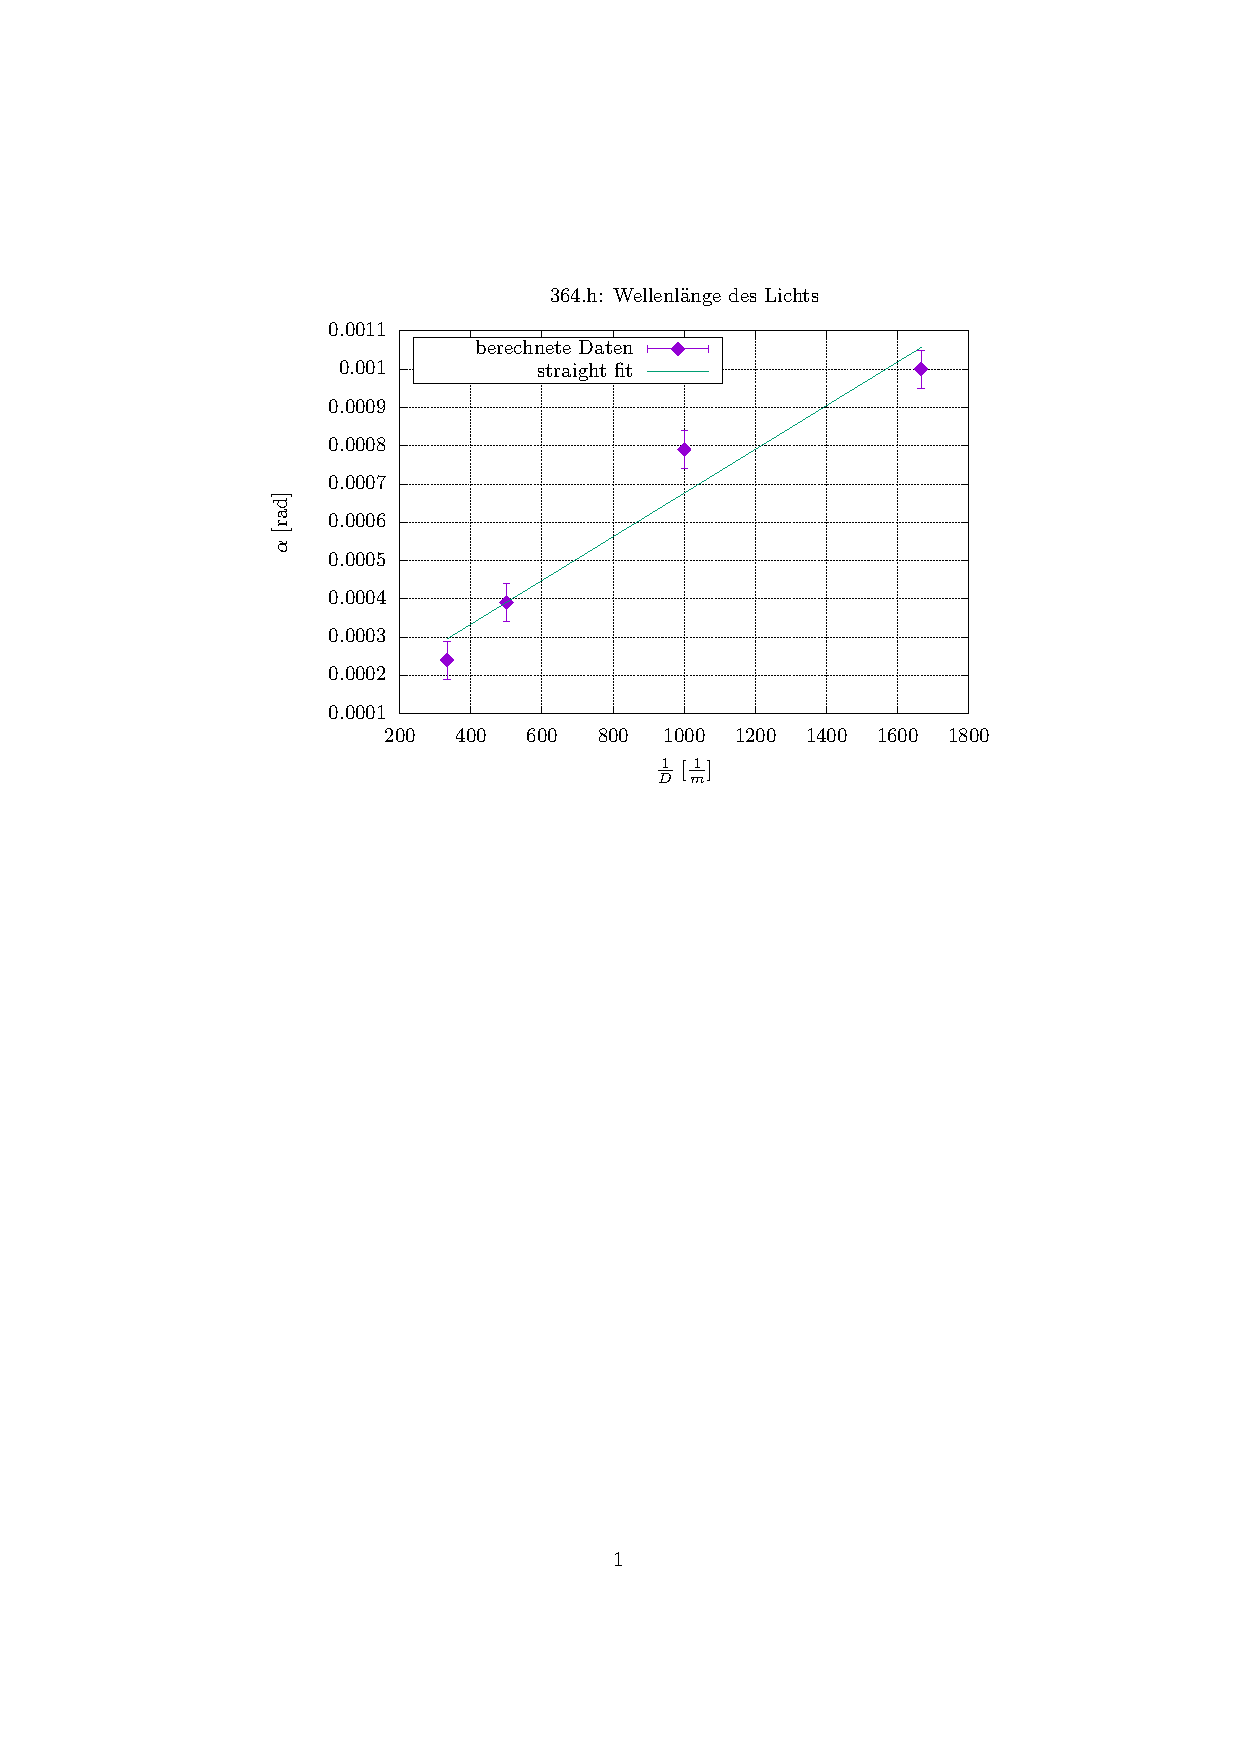
\includegraphics[width=\textwidth]{plots/plot.pdf}
    \captionof{figure}{The Fermi-Dirac and Bose-Einstein distributions for the respective chemical potential $\mu _f$ and $\mu _b$.
    $f(\varepsilon _i)(1-f(\varepsilon _i))=\text{Var}(n_i)$} \label{fig:fermi bose distribution}
\end{Figure}

With this information one can also calculate the mean particle number in the system
\begin{align} 
  \left\langle N\right\rangle  &= \sum_{i}^{}\left\langle n_i\right\rangle \!(E_i)\\
                               &= \int_{}^{}\td E\rho (E)\left\langle n_i\right\rangle \!(E)
,\end{align} 
where $\left\langle n_i\right\rangle \!(E)$ specifies that a energy dependent distribution is needed.
The integral form with the density of states is valid for when the energy levels are close enough.
If the particle number is fixed then $\left\langle N\right\rangle =N$.
%}}}

%{{{ Fermi-Dirac Statistics
\subsection{Fermi-Dirac Statistics}
For Fermions $n_i  \in \left[0,1\right]$ thus
\begin{align} 
  \mathcal{Z}=\prod_{i}^{}\left(1+\text{e}^{\alpha -\beta \varepsilon _i}\right)
.\end{align} 
The average occupation number for a single energy level $i$ is calculated via 
\begin{align} 
  \left\langle n_i\right\rangle  &= \sum_{ \left\{n\right\}}^{}p_i n_i\\
                                 &= \sum_{ \left\{n\right\}}^{}\dfrac{1}{\mathcal{Z}}\text{e}^{(\alpha -\beta \varepsilon _i)n_i}n_i\\
                                 &= \sum_{ \left\{n\right\}}^{}\dfrac{\text{e}^{(\alpha -\beta \varepsilon _i)n_i}n_i}{\sum_{ \left\{n\right\}}^{}\text{e}^{(\alpha -\beta \varepsilon _i)n_i}}
\end{align} 
all sums $\sum_{n_j}^{}\hdots \sum_{n_k}^{}$ that are not about $n_i$ will cancel with the partition function
\begin{align} 
  \left\langle n_i\right\rangle  &= \dfrac{\sum_{n_i}^{}\text{e}^{(\alpha -\beta \varepsilon _i)n_i}n_i}{\sum_{n_i}^{}\text{e}^{(\alpha -\beta \varepsilon _i)n_i}}\\
                                 &= \dfrac{0+\text{e}^{\alpha -\beta \varepsilon _i}}{1+\text{e}^{\alpha -\beta \varepsilon _i}}\\
                                 &= \dfrac{1}{\text{e}^{-(\alpha -\beta \varepsilon _i)}+1}\\
                                 &= \boxed{\dfrac{1}{\text{e}^{\tfrac{\varepsilon _i-\mu }{k_BT}}+1} =: f(\varepsilon _i)}
.\end{align} 
This is the Fermi distribution.
It holds not only for the single energy level $i$ but more generally for the whole system.

The variance is given by
\begin{align} 
  \text{Var}(n_i) &= \left\langle n_i^2\right\rangle -\left\langle n_i\right\rangle ^2\\
                  &= \left\langle n_i\right\rangle -\left\langle n_i\right\rangle \left\langle n_i\right\rangle \\
                  &= f(\varepsilon _i)(1-f(\varepsilon _i))
,\end{align} 
since $n_i^2=n_i$ for Fermions.

The distribution has a width of $2k_BT$ and is centered on $\mu $.
For $f(\varepsilon _i<\mu )\rightarrow 1$ and $f(\varepsilon _i>\mu )\rightarrow 0$.
At $f(\varepsilon _i=\mu )=0.5$.

An interesting property arises for $T\rightarrow 0$.
$f(\varepsilon _i)$ will then be infinitely sharp around $\mu $ since the width is proportional to $T$, s.t.\ 
\begin{align} 
  \lim_{T\rightarrow 0}f(\varepsilon _i)=\theta (\mu -\varepsilon _i)
.\end{align}
As a consequence for the low temperature regime the only states which can be occupied are for energies $\varepsilon _i<\mu $.
This energy is also called the Fermi energy $\mu (T=0)=\varepsilon _F$.
The corresponding momentum is the Fermi momentum $p_F=\tfrac{\varepsilon _F}{2m}$.
The Fermi energy is calculated with the particle number for $T\rightarrow 0$.
Consider a free fermionic gas with quadradic dispersion relation $E=\tfrac{p^2}{2m}$
\begin{align} 
  \rho  &= \int_{}^{}\td \Gamma \,\delta \left(E-E_f\right)\\
        &= \dfrac{V}{(2\pi \hbar )^3}\int_{}^{}\td S_2\,\int_{}^{}\td p\,p^2\delta (E-E_f)\\
        &= \dfrac{V}{2\pi ^2\hbar ^3}\int_{}^{}\td E\,\dfrac{m\cdot 2mE}{\,\sqrt[]{2mE}}\delta (E-E_f)\\
        &= V\dfrac{m\,\sqrt[]{2m}}{2\pi ^2\hbar ^3}\,\sqrt[]{E} =: Vc \,\sqrt[]{E}
.\end{align} 
The average particle number is thus
\begin{align} 
  \left\langle N\right\rangle &= \left\langle \sum_{i}^{}n_i\right\rangle =\sum_{i}^{}\left\langle n_i\right\rangle \\
                              &= \sum_{i}^{}f(\varepsilon _i) = \int_{}^{}\td E\,\rho (E)f(E)\\
                              &\stackrel{T\rightarrow 0}{=} Vc\int_{0}^{\varepsilon _F}\td E\,\,\sqrt[]{E}\\
                              &= Vc \dfrac{2}{3}\varepsilon _F^{3/2}\\
  \Leftrightarrow \varepsilon _F &= \left(\dfrac{3}{2}\dfrac{\left\langle N\right\rangle }{Vc}\right)^{\tfrac{2}{3}}
.\end{align} 
%}}}

%{{{ Bose-Einstein Statistics
\subsection{Bose-Einstein Statistics}
For Bosons $n_i  \in [0,\infty)$ thus
\begin{align} 
  \mathcal{Z} &= \prod_{i}^{}\sum_{n_i}^{}\text{e}^{(\alpha -\beta \varepsilon _i)n_i}
.\end{align} 
Consider
\begin{align} 
  \text{e}^{\alpha -\beta \varepsilon _i}&<1\\
  \Leftrightarrow \alpha -\beta \varepsilon _i&<0\\
  \Leftrightarrow \mu &<\varepsilon _i
\end{align} 
which is always the case for Bosons.
The physical interpretation is that a system of Bosons has no restrictions in which state a new Boson can go and thus will in general increase its energy with the additions $(\mu <0)$ or at most nothing will happen $(\mu =0)$\footnote{This is the case for photons.}.
If this constraint holds then the sum will converge
\begin{align} 
  \mathcal{Z} &= \prod_{i}^{}\dfrac{1}{1-\text{e}^{\alpha -\beta \varepsilon _i}}=\prod_{i}^{}\mathcal{Z}_i
.\end{align} 

The average occupation number for a single energy level $i$ is calculated via
\begin{align} 
  \left\langle n_i\right\rangle  &= \sum_{ \left\{n\right\}}^{}p_i n_i\\
                                 &= \sum_{ \left\{n\right\}}^{}\dfrac{1}{\mathcal{Z}}\text{e}^{(\alpha -\beta \varepsilon _i)n_i}n_i\\
                                 &= \sum_{ \left\{n\right\}}^{}\dfrac{\text{e}^{(\alpha -\beta \varepsilon _i)n_i}n_i}{\sum_{ \left\{n\right\}}^{}\text{e}^{(\alpha -\beta \varepsilon _i)n_i}}
\end{align} 
all sums $\sum_{n_j}^{}\hdots \sum_{n_k}^{}$ that are not about $n_i$ will cancel with the partition function
\begin{align} 
  \left\langle n_i\right\rangle  &= \dfrac{\sum_{n_i}^{}\text{e}^{(\alpha -\beta \varepsilon _i)n_i}n_i}{\sum_{n_i}^{}\text{e}^{(\alpha -\beta \varepsilon _i)n_i}}\\
                                 &= \diffp[]{\ln\left(\sum_{n_i}^{}\text{e}^{(\alpha -\beta \varepsilon _i)n_i}\right)}{(\alpha -\beta \varepsilon _i)}\\
                                 &= \diffp[]{\ln \mathcal{Z}_i}{(\alpha -\beta \varepsilon _i)}\\
                                 &= -\diffp[]{\ln \left(1-\text{e}^{\alpha -\beta \varepsilon _i}\right)}{(\alpha -\beta \varepsilon _i)}\\
                                 &= \dfrac{\text{e}^{\alpha -\beta \varepsilon _i}}{1-\text{e}^{\alpha -\beta \varepsilon _i}}\\
                                 &=\dfrac{1}{\text{e}^{-(\alpha -\beta \varepsilon _i)}-1}\\
                                 &=\boxed{\dfrac{1}{\text{e}^{\tfrac{\varepsilon _i-\mu }{k_BT}}-1}=:b(\varepsilon _i)}
.\end{align} 
This is the Bose distribution.
It holds not only for the single energy level $i$ but more generally for the whole system.

These distributions are quite similar and only differ by a sign; plus for Fermions and minus for Bosons.

TODO BEC
%}}}

%{{{ Grand Canonical Ensemble
\subsection{Grand Canonical Ensemble}
Since the partition sums are quite similar
\begin{align} 
  \mathcal{Z}_f &= \prod_{i}^{}\left(1+\text{e}^{-\beta (\varepsilon _i-\mu )}\right)\\
  \mathcal{Z}_b &= \prod_{i}^{}\dfrac{1}{1-\text{e}^{-\beta (\varepsilon _i-\mu )}}
,\end{align} 
the grand canonical potential is given by
\begin{align} 
  \Phi  &= -k_BT\ln\mathcal{Z} \\
        &= \mp k_BT\sum_{i}^{}\ln \left(1\pm\text{e}^{-\beta (\varepsilon _i-\mu )}\right)\\
        &= \mp k_BT\int_{}^{}\td \varepsilon \,\rho (\varepsilon )\ln \left(1\pm\text{e}^{-\beta (\varepsilon _i-\mu )}\right)
,\end{align} 
with the top row for fermions and the bottom row for bosons.
%}}}

%}}}

%{{{ Phase Transitions
\section{Phase Transitions}
In thermodynamical / statistical systems the behaviour of particles has been regarded as non-interacting.
This leads to thermodynamic functions, which depend on the properties (e.g.\ energy) of the single particles and produces accurate results.
However, if one allows for the interaction of particles to happen, a collective, long-range behaviour of the system arises.
This can be seen at certain temperatures, when so called phase transistion occur.
A phase transition is a transistion for which a certain order parameter $m$ has a zero value and now takes a non-zero value (throughout the whole medium, thus long-range).
Such order parameters can be for example the magnetisation of a medium.
The need for these parameters arises, as a phase transition breaks the symmetry of the system and introduces a new variable which is needed to describe the system in its current state.

%{{{ Order Parameter \& Critical Exponents
\subsection{Order Parameter \& Critical Exponents}
First order phase transitions involve a latent heat.
This heat is absorbed or released during a phase transition while the system stays at constant temperature.
I.e.\ this heat is the energy needed (or released) in the phase transition.
In the process there can be multiple phases present (also called mixed-phase-regime) when some parts of the system have transitioned and other parts not.
A prominent example is the phase transition of solid water to liquid water.

Second order phase transitions involve the divergence of the susceptibility (i.e.\ linear response functions or the second derivative of a thermodynamic potential).
This is seen in the transition of a ferromagnetic material to a paramagnetic material at a critical temperature.

A phase transition is of $n$-th order when 
\begin{align} 
  \diffp[n]{F}{X}\qquad \text{diverges}
.\end{align} 
Here $F$ is the thermodynamic potential (free energy generally) and $X$ is a state variable (intensive generally).
For example in the $2^\text{nd}$ order with 
\begin{align} 
  \td F=-S\td T+M\td B
\end{align} 
then
\begin{align} 
  \left(\diffp[2]{F}{B}\right)_T=\left(\diffp[]{M}{B}\right)_T=\chi 
\end{align} 
diverges at the Curie-temperature in the phase transition of a ferromagnet to a paramagnet.
More generally one can define the order parameter $m$ and an ordering field $h$, s.t.\ in the limit of $h\rightarrow 0$, $m$ tends to a limiting value $m_0$ which is zero for $T\geq T_c$ and non-zero for $T<T_c$.

The intrinsic measures of the system are not sufficient in describing the phase transition since the correlation length $\xi $ extends to infinity.
Thus one needs a measure of the phase transition which is length/scale independent.
The only functions which fulfill this criterium are polynomials
\begin{align} 
  f(x) = x^\alpha \rightarrow f(x) &= (Ax)^\alpha \\
  \Leftrightarrow \dfrac{f(x)}{A^\alpha } &= x^\alpha \\
  \Leftrightarrow f^*(x) &= x^\alpha 
.\end{align} 
Thus at the critical temperature the defining properties of the phase transition are described by polynomials or the power law.
The way the order parameter vanishes at the critical temperature is defined by
\begin{align} 
  m_0\propto \left|\dfrac{T-T_c}{T_c}\right|^\beta =|\tau |^\beta 
,\end{align} 
where $\beta $ is the critical exponent and 
\begin{align} 
  \dfrac{T-T_c}{T_c}=:\tau 
\end{align} 
is the reduced temperature.
For the ordered phase $\tau <0$, for the disordered phase $\tau >0$ and at the critical temperature $\tau =0$.
The susceptibilities are defined equally
\begin{align} 
  \chi  &\propto \left.\diffp[]{m}{h}\right|_{h\rightarrow 0}\propto \begin{cases}
    \tau ^{-\gamma }\, \text{above}\\
    (-\tau )^{-\gamma '} \, \text{below}\\
  \end{cases}\\
  c_V &\propto \begin{cases}
    \tau ^{-\alpha }\, \text{above}\\
    (-\tau )^{-\alpha '}\, \text{below}
  \end{cases}
,\end{align} 
for $\chi $ the magnetic susceptibility with $m=M$ the magnetisation, $h=B$ the external magnetic field and $c_V$ the specific heat capacity.

In general the usage of the label of the critical exponents is not arbitrary.
To summarize:
$\alpha $ relates the specific heat to the temperature $c_V\propto|\tau |^{-\alpha }$; $\beta $ relates the order parameter to the temperature $m\propto|\tau |^{\beta }$; $\gamma $ relates the systems response / susceptibility to an external driving parameter (exeternal field) $\chi \propto\diffp[]{m}{h}\propto|\tau |^{-\gamma }$
\footnote{There are many more critical exponents relating the order parameter or other various quantities of the system with the temperature.
These are not listed here (see a summary on wikipedia on the article of universality classes).}.

Different systems who share the same critical exponents behave identical at the critical temperature.
Thus a certain set of critical exponents is called a universality class and all systems belonging to this class show the same behaviour at the critical temperature.
If a model solves a given system (i.e.\ yields a set of critical exponents), then other systems solved with this model will belong to the same universality class and thus behave the same way at $T_c$.
%}}}

%{{{ Ising Model
\subsection{Ising Model}
TODO SEE NOTES ON PAPER
%}}}

%}}}

\end{multicols}

%\clearpage
%\listoffigures
%\listoftables
%\bibliographystyle{plain}
%\bibliography{refs}

\end{document}
